\documentclass[aspectratio=169]{beamer}
\usepackage{tikz}
\usetikzlibrary{calc}
\usetikzlibrary{backgrounds}
\usetikzlibrary{arrows.meta}


% Theme and layout
\usetheme{Madrid}
\useoutertheme{infolines} % shows current section in the header and slide numbers in the footer
\setbeamertemplate{navigation symbols}{} % hide nav icons
\usepackage{pgfplots} % illustrations
\pgfplotsset{compat=1.18} % illustrations
\usetikzlibrary{calc} % tikz calculations
\usepackage{subcaption} % for subfigures
\usetikzlibrary{positioning, arrows.meta, calc, decorations.pathmorphing, decorations.markings, shapes.geometric}
\usetikzlibrary{decorations.pathreplacing} % For braces

\usepackage{amsmath}   % For \text{} in math mode and general math improvements
\usepackage{amssymb}   % For \mathbb{} (like the E for Expectation)
\usepackage{xcolor}    % For using \color{red}
\usetikzlibrary{backgrounds}
\usepackage{pifont}
\usepackage{adjustbox}

% Metadata
\title{Optimistic and Pessimistic Algorithms}
\author{Sebastian Reboul \hspace{4cm}}
\date{Séminaire Doctorant TSP}

\tikzset{axis/.style={->, -{Stealth}, line width=0.6pt}}

\begin{document}

\frame{\titlepage}

\begin{frame}
  \begin{figure}
    \centering
    
\includegraphics[width=0.6\textwidth]{octopus.png}
  \end{figure}
\end{frame}

\input|"./.venv/bin/python -u scripts/mab_problem.py"


\begin{frame}{Regret}

\begin{block}{\centering Measuring Learning Performance}
\begin{itemize}
    \item Regret quantifies how much reward the learner \textit{misses out on}
          compared to the best fixed action in hindsight.
    \item For a horizon $T$:
    \[
    R_T = T\mu^* - \mathbb{E}\!\left[\sum_{t=1}^T \mu_{A_t}\right]
    \]
    \item $\mu^*$: expected reward of the optimal arm.  
          $\mu_{A_t}$: expected reward of chosen arm $A_t$.
    \item Small regret $\Rightarrow$ the learner performs nearly as well as the best arm.
\end{itemize}
\end{block}

\vspace{0.6em}
\pause
\centering
\textcolor{gray!70}{Our goal is to make this difference --- the regret --- as small as possible.}
\end{frame}

\begin{frame}[fragile]
\frametitle{Visuals Explained}
\begin{figure}
    \centering
    \resizebox{0.8\textwidth}{!}{
        % This is the final, complete version of the graphic.
% It includes mathematical definitions and clarifies the context of the analysis.
% The canvas size and drawing order are correct to ensure proper scaling and appearance.

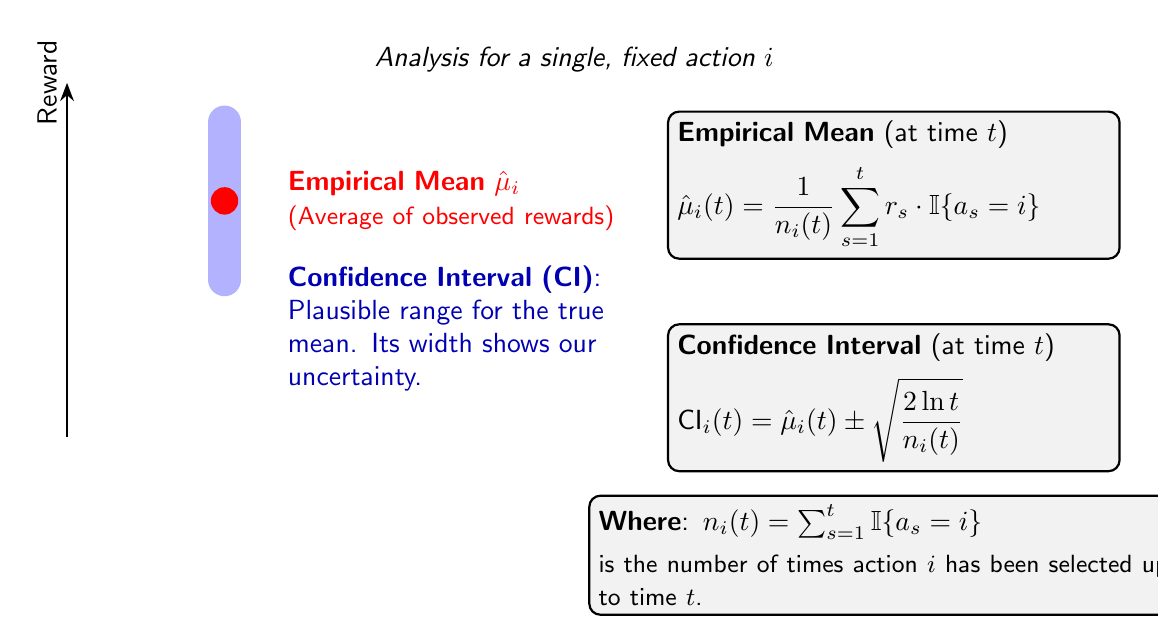
\begin{tikzpicture}[
    font=\sffamily,
    ci_bar/.style={line width=12pt, cap=round, blue!60, opacity=0.5},
    mean_dot/.style={circle, fill=red, inner sep=3.5pt},
    axis/.style={->, >=Stealth, thick},
    formula_box/.style={draw, thick, rounded corners, fill=gray!10, align=left}
]

% --- Bounding Box to guarantee correct size and scaling ---
\useasboundingbox (1, -2) rectangle (15, 5.2);


% --- Subtitle for context ---
% Appears on slide 2 to explain that this is a per-action analysis.
\onslide<2->{
    \node[font=\sffamily\itshape, align=center] at (8, 4.8) {
        Analysis for a single, fixed action $i$
    };
}

% --- SLIDE 1: The Axis ---
\onslide<1->{
    \draw[axis] (1.5, 0) -- (1.5, 4.5) node[above, rotate=90, anchor=south] {Reward};
}

% --- SLIDE 3: The Confidence Interval BAR ---
% The BAR is drawn on slide 3, in the background.
\onslide<3->{
    \draw[ci_bar] (3.5, 2.0) -- (3.5, 4.0);
}

% --- SLIDE 2: The Empirical Mean (Dot and Text) ---
% The DOT and its text appear on slide 2, drawn on top of the bar on slide 3.
\onslide<2->{
    \node (mean_dot) [mean_dot] at (3.5, 3.0) {};
    \node (mean_text) [text width=4.5cm, align=left, anchor=west, right=0.5cm of mean_dot] {
        \textcolor{red}{
            \textbf{Empirical Mean} $\hat{\mu}_i$ \\
            \small(Average of observed rewards)
        }
    };
}

% --- SLIDE 3: The Confidence Interval TEXT ---
% The TEXT for the CI appears on slide 3.
\onslide<3->{
    \node [text width=4.5cm, align=left, anchor=north west, below=0.2cm of mean_text] {
        \textcolor{blue!70!black}{
             \textbf{Confidence Interval (CI)}: Plausible range for the true mean. Its width shows our uncertainty.
        }
    };
}

% --- MATHEMATICAL FORMULAS (on the right) ---

% --- SLIDE 2: Empirical Mean Formula ---
\onslide<2->{
    \node[formula_box, text width=5.5cm] at (12, 3.2) {
        \textbf{Empirical Mean} (at time $t$) \\[5pt]
        $\displaystyle \hat{\mu}_i(t) = \frac{1}{n_i(t)} \sum_{s=1}^{t} r_s \cdot \mathbb{I}\{a_s = i\}$
    };
}

% --- SLIDE 3: Confidence Interval Formula ---
\onslide<3->{
     \node[formula_box, text width=5.5cm] at (12, 0.5) {
         \textbf{Confidence Interval} (at time $t$) \\[5pt]
         $\displaystyle \text{CI}_i(t) = \hat{\mu}_i(t) \pm \sqrt{\frac{2 \ln t}{n_i(t)}}$
     };
}

% --- Definition of n_i(t) ---
% Appears with the first formula that uses it (on slide 2).
\onslide<2->{
    \node[formula_box, text width=7.5cm] at (12, -1.5) {
        \textbf{Where}: $n_i(t) = \sum_{s=1}^t \mathbb{I}\{a_s = i\}$ \\[3pt]
        \small is the number of times action $i$ has been selected up to time $t$.
    };
}

\end{tikzpicture}
    }
\end{figure}
\end{frame}

\input|"./.venv/bin/python -u scripts/eac_beamer.py"

\input|"./.venv/bin/python -u scripts/ae_beamer.py"

\input|"./.venv/bin/python -u scripts/ucb_beamer.py"

\begin{frame}{What is a Regret Bound?}

\begin{block}{\centering Bounding the Learning Loss}
\begin{itemize}
    \item A \textbf{regret bound} tells us how large the regret can grow as $T$ increases.
    \item We say an algorithm satisfies
    \[
    R_T \leq C\,f(T)
    \]
    for some function $f(T)$ and constant $C>0$.
    \item This means the algorithm’s regret is \textit{no worse than} the rate $f(T)$.
    \item Example growth rates:
    \[
    \mathcal{O}(\sqrt{T}), \quad \mathcal{O}(T^{2/3}), \quad \mathcal{O}(T)
    \]
    \item The smaller the bound, the faster the algorithm learns.
\end{itemize}
\end{block}

\vspace{0.5em}
\pause
\centering
\textcolor{gray!70}{A good algorithm keeps $R_T$ \textbf{below} its theoretical upper bound for all $T$.}

\end{frame}


\begin{frame}[fragile]
\frametitle{Theoretical Regret Bounds}
\begin{figure}
    \centering
    % slides/regret_comparison.tex
\begin{figure}[H]
\centering
\resizebox{0.92\textwidth}{!}{%
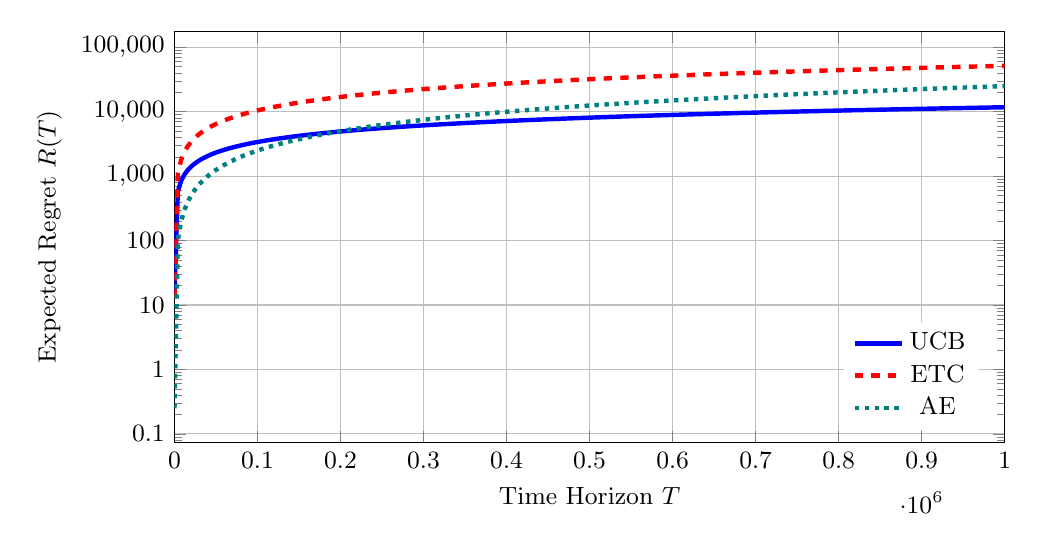
\begin{tikzpicture}
\pgfmathsetmacro{\K}{10}

\begin{semilogyaxis}[
    width=\textwidth,
    height=6.8cm,
    samples=250,
    domain=10:1e6,
    xmin=10, xmax=1e6,
    xlabel={Time Horizon $T$},
    ylabel={Expected Regret $R(T)$},
    legend style={
        at={(0.97,0.03)},
        anchor=south east,
        font=\small,
        fill=white,
        draw=none
    },
    grid=major,
    log ticks with fixed point,
    tick label style={font=\small},
    label style={font=\small},
]

    % --- UCB: O(sqrt(K T log T)) ---
    \addplot[ultra thick, blue] {sqrt(\K*x*ln(x))};
    \addlegendentry{UCB}

    % --- ETC (untuned): ~O(K^{1/3} T^{2/3}) ---
    \addplot[ultra thick, dashed, red] {(\K)^(1/3)*(x)^(2/3)*(ln(x))^(1/3)};
    \addlegendentry{ETC}

    % --- AE (fixed budget): O(T) ---
    \addplot[ultra thick, dotted, teal] {0.025*x};
    \addlegendentry{AE}

\end{semilogyaxis}
\end{tikzpicture}%
}
\end{figure}

\end{figure}
\end{frame}

% --- Offline Multi-Armed Bandit Setup ---
\begin{frame}{Offline Multi-Armed Bandit Setup}

\begin{block}{Offline Data Collection}
\begin{itemize}
    \item Unlike the online setting, the learner cannot interact with the environment.
    \item Instead, it receives a fixed dataset
    \[
    \mathcal{D} = \{(a_i, r_i)\}_{i=1}^{N}
    \]
    collected by a \textbf{behavior policy} $\beta(a)$.
    \item Each arm $a$ is sampled with probability $\beta(a)$, and rewards $r_i$ are drawn from the true reward distribution of that arm.
\end{itemize}
\end{block}

\pause
\begin{block}{Learning Objective}
\begin{itemize}
    \item Using only $\mathcal{D}$, estimate an arm $\hat{a}$ (or policy $\hat{\pi}$) that maximizes expected reward.
    \item Evaluate performance via the \textbf{offline regret:}
    \[
    R_{\text{off}} = \mu^* - \mathbb{E}_{\mathcal{D}}[\,\mu_{\hat{a}}\,].
    \]
\end{itemize}
\end{block}

\end{frame}


% --- Comparing Online vs Offline Regret ---
\begin{frame}{Online vs Offline Regret}

\begin{columns}[T,onlytextwidth]
\column{0.48\textwidth}
\begin{block}{\centering Online Bandit}
\begin{itemize}
    \item Learner interacts with environment.
    \item Chooses $A_t$, observes reward $r_t$.
    \item \textbf{Regret:}
    \[
    R_T = T\mu^* - \mathbb{E}\!\left[\sum_{t=1}^T \mu_{A_t}\right]
    \]
    \item Goal: \textit{learn while acting.}
\end{itemize}
\end{block}

\column{0.48\textwidth}
\begin{block}{\centering Offline Bandit}
\begin{itemize}
    \item Learner receives fixed dataset $\mathcal{D}$.
    \item No further interaction.
    \item \textbf{Regret:}
    \[
    R_{\text{off}} = \mu^* - \mathbb{E}_{\mathcal{D}}[\,\mu_{\hat{a}}\,]
    \]
    \item Goal: \textit{learn from logged data.}
\end{itemize}
\end{block}
\end{columns}

\vspace{0.8em}
\pause
\centering
\textcolor{gray!70}{Both measure performance loss — but online regret arises from exploration, while offline regret stems from limited data coverage.}

\end{frame}

\input|"./.venv/bin/python -u scripts/offline_rl_beamer.py"

% --- The Concentrability Coefficient C* ---
\begin{frame}{Understanding $C^*$ in Multi-Armed Bandits}

\begin{block}{Definition}
In offline bandit problems, the dataset is collected under a \textbf{behavior policy} $\beta(a)$,
while the goal is to identify the \textbf{optimal arm} $a^*$ with mean reward $\mu_{a^*}$.
The \textbf{concentrability coefficient} $C^*$ is defined as:
\[
\frac{1}{\beta(a^*)} \le C^*
\]
It measures how well the data distribution $\beta(a)$ covers the optimal arm $a^*$.
\end{block}

\pause
\begin{block}{Intuition}
\begin{itemize}
    \item $C^* = 1$ : dataset perfectly matches the optimal arm (expert data).
    \item $C^* > 1$ : suboptimal arms appear more often — weaker coverage of $a^*$.
    \item Larger $C^*$ $\Rightarrow$ greater distribution mismatch, harder learning.
\end{itemize}
\end{block}

\end{frame}

% --- Visualizing the Role of C* ---
\begin{frame}{Effect of $C^*$ on Offline Learning}

\centering
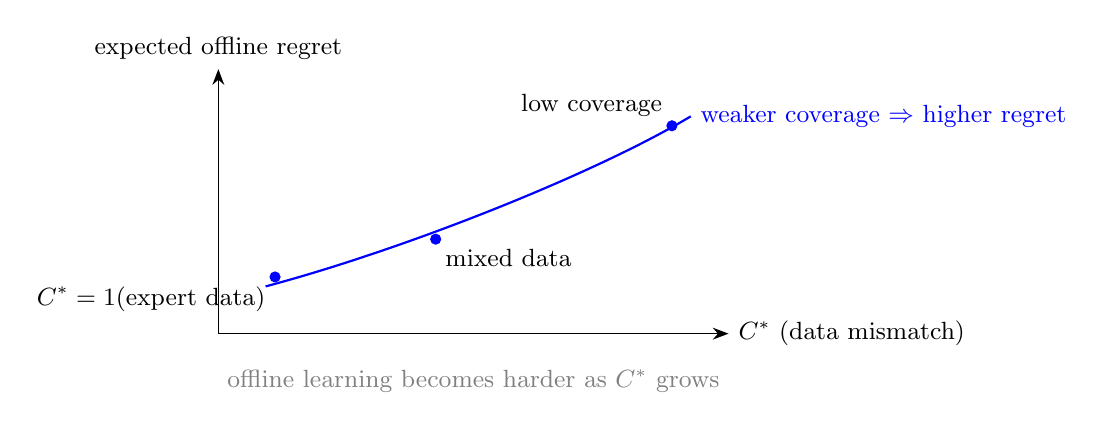
\begin{tikzpicture}[scale=1.2, every node/.style={font=\small}]
    % Axes
    \draw[axis] (0,0) -- (5.4,0) node[right] {$C^*$ (data mismatch)};
    \draw[axis] (0,0) -- (0,2.8) node[above] {expected offline regret};

    % Curve
    \draw[thick, blue] (0.5,0.5) .. controls (2,0.9) and (4,1.7) .. (5,2.3);
    \node[blue, right] at (5,2.3) {weaker coverage $\Rightarrow$ higher regret};

    % Points and labels
    \filldraw[blue] (0.6,0.6) circle (1.5pt);
    \node[below left] at (0.6,0.6) {$C^* = 1$ \\ (expert data)};

    \filldraw[blue] (2.3,1.0) circle (1.5pt);
    \node[below right] at (2.3,1.0) {mixed data};

    \filldraw[blue] (4.8,2.2) circle (1.5pt);
    \node[above left] at (4.8,2.2) {low coverage};

    % Annotation
    \node[gray] at (2.7,-0.5) {offline learning becomes harder as $C^*$ grows};
\end{tikzpicture}

\vspace{1em}
\pause
\textcolor{gray!70}{Smaller $C^*$ means better overlap between $\beta(a)$ and the optimal arm — \\ leading to faster convergence and lower offline regret.}
\end{frame}

\begin{frame}
  \begin{figure}
    \centering
    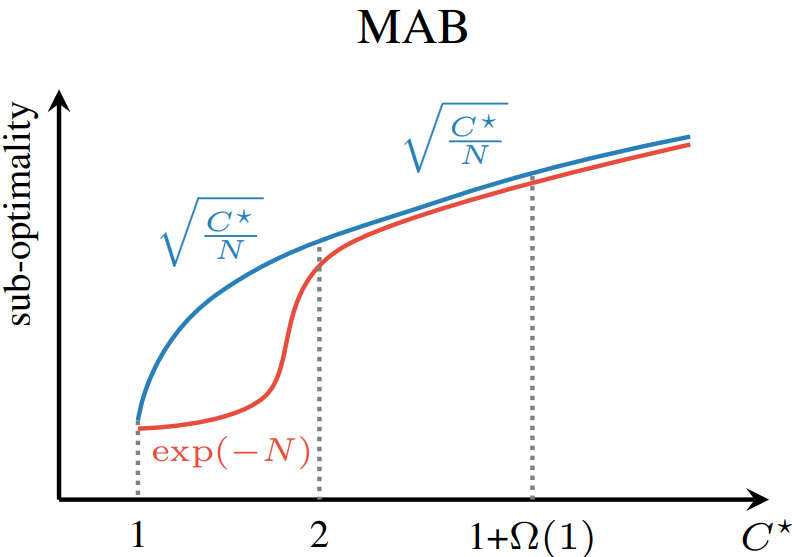
\includegraphics[width=0.5\textwidth]{mabs.png}
  \end{figure}
\end{frame}

% File: rl_as_stacked_mab.tex
% A single slide illustrating Reinforcement Learning as a sequence of Multi-Armed Bandit problems.
% To be included in a main Beamer presentation using % File: rl_as_stacked_mab.tex
% A single slide illustrating Reinforcement Learning as a sequence of Multi-Armed Bandit problems.
% To be included in a main Beamer presentation using % File: rl_as_stacked_mab.tex
% A single slide illustrating Reinforcement Learning as a sequence of Multi-Armed Bandit problems.
% To be included in a main Beamer presentation using \input{rl_as_stacked_mab.tex}

\begin{frame}{Reinforcement Learning as Stacked Bandits}
\frametitle{From Bandits to Reinforcement Learning}

\begin{figure}[h]
    \centering
    \begin{tikzpicture}[
        % Style for nodes containing the octopus image
        bandit/.style={
            inner sep=0, % No extra padding around the image
        },
        % Style for the arrows connecting the bandit problems
        arrow/.style={
            -latex,      % Use LaTeX arrow tip
            thick,       % Make the line thick
            draw=blue!70, % A nice blue color
            shorten <=2pt, % Shorten start of arrow slightly
            shorten >=2pt, % Shorten end of arrow slightly
        },
        % Style for the labels on the arrows
        label/.style={
            midway,      % Position label in the middle of the path
            above,       % Position label above the path
            font=\small, % Use a small font size
            fill=white,  % Give it a white background to stand out
            inner sep=1pt, % A little padding around the text
        }
    ]
        % Node 1: The first bandit problem (state s_1)
        % This node appears on all slides of the frame.
        \node<1->[bandit] (img1) {
\includegraphics[width=0.2\textwidth]{octopus.png}};
        \node[below=1pt of img1] {$s_1$};

        % Node 2: The second bandit problem (state s_2)
        % This node appears from the second slide onwards.
        \node<2->[bandit, right=3cm of img1] (img2) {
\includegraphics[width=0.2\textwidth]{octopus.png}};
        \node<2->[below=1pt of img2] {$s_2$};

        % Node 3: The third bandit problem (state s_3)
        % This node appears from the third slide onwards.
        \node<3->[bandit, right=3cm of img2] (img3) {
\includegraphics[width=0.2\textwidth]{octopus.png}};
        \node<3->[below=1pt of img3] {$s_3$};

        % Dots to indicate the sequence continues...
        % This appears from the fourth slide onwards.
        \node<4->[right=2cm of img3] (dots) {\Huge \dots};

        % Arrow 1: From s_1 to s_2
        % This appears on the second slide onwards.
        \draw<2->[arrow] (img1) -- (img2) node[label] {action $a_1$, get reward $r_1$};

        % Arrow 2: From s_2 to s_3
        % This appears on the third slide onwards.
        \draw<3->[arrow] (img2) -- (img3) node[label] {action $a_2$, get reward $r_2$};

    \end{tikzpicture}
    \caption{In RL, the action chosen in the current state (a bandit problem) determines the next state (a new bandit problem).}
\end{figure}

\end{frame}

\begin{frame}{Reinforcement Learning as Stacked Bandits}
\frametitle{From Bandits to Reinforcement Learning}

\begin{figure}[h]
    \centering
    \begin{tikzpicture}[
        % Style for nodes containing the octopus image
        bandit/.style={
            inner sep=0, % No extra padding around the image
        },
        % Style for the arrows connecting the bandit problems
        arrow/.style={
            -latex,      % Use LaTeX arrow tip
            thick,       % Make the line thick
            draw=blue!70, % A nice blue color
            shorten <=2pt, % Shorten start of arrow slightly
            shorten >=2pt, % Shorten end of arrow slightly
        },
        % Style for the labels on the arrows
        label/.style={
            midway,      % Position label in the middle of the path
            above,       % Position label above the path
            font=\small, % Use a small font size
            fill=white,  % Give it a white background to stand out
            inner sep=1pt, % A little padding around the text
        }
    ]
        % Node 1: The first bandit problem (state s_1)
        % This node appears on all slides of the frame.
        \node<1->[bandit] (img1) {
\includegraphics[width=0.2\textwidth]{octopus.png}};
        \node[below=1pt of img1] {$s_1$};

        % Node 2: The second bandit problem (state s_2)
        % This node appears from the second slide onwards.
        \node<2->[bandit, right=3cm of img1] (img2) {
\includegraphics[width=0.2\textwidth]{octopus.png}};
        \node<2->[below=1pt of img2] {$s_2$};

        % Node 3: The third bandit problem (state s_3)
        % This node appears from the third slide onwards.
        \node<3->[bandit, right=3cm of img2] (img3) {
\includegraphics[width=0.2\textwidth]{octopus.png}};
        \node<3->[below=1pt of img3] {$s_3$};

        % Dots to indicate the sequence continues...
        % This appears from the fourth slide onwards.
        \node<4->[right=2cm of img3] (dots) {\Huge \dots};

        % Arrow 1: From s_1 to s_2
        % This appears on the second slide onwards.
        \draw<2->[arrow] (img1) -- (img2) node[label] {action $a_1$, get reward $r_1$};

        % Arrow 2: From s_2 to s_3
        % This appears on the third slide onwards.
        \draw<3->[arrow] (img2) -- (img3) node[label] {action $a_2$, get reward $r_2$};

    \end{tikzpicture}
    \caption{In RL, the action chosen in the current state (a bandit problem) determines the next state (a new bandit problem).}
\end{figure}

\end{frame}

\begin{frame}{Reinforcement Learning as Stacked Bandits}
\frametitle{From Bandits to Reinforcement Learning}

\begin{figure}[h]
    \centering
    \begin{tikzpicture}[
        % Style for nodes containing the octopus image
        bandit/.style={
            inner sep=0, % No extra padding around the image
        },
        % Style for the arrows connecting the bandit problems
        arrow/.style={
            -latex,      % Use LaTeX arrow tip
            thick,       % Make the line thick
            draw=blue!70, % A nice blue color
            shorten <=2pt, % Shorten start of arrow slightly
            shorten >=2pt, % Shorten end of arrow slightly
        },
        % Style for the labels on the arrows
        label/.style={
            midway,      % Position label in the middle of the path
            above,       % Position label above the path
            font=\small, % Use a small font size
            fill=white,  % Give it a white background to stand out
            inner sep=1pt, % A little padding around the text
        }
    ]
        % Node 1: The first bandit problem (state s_1)
        % This node appears on all slides of the frame.
        \node<1->[bandit] (img1) {
\includegraphics[width=0.2\textwidth]{octopus.png}};
        \node[below=1pt of img1] {$s_1$};

        % Node 2: The second bandit problem (state s_2)
        % This node appears from the second slide onwards.
        \node<2->[bandit, right=3cm of img1] (img2) {
\includegraphics[width=0.2\textwidth]{octopus.png}};
        \node<2->[below=1pt of img2] {$s_2$};

        % Node 3: The third bandit problem (state s_3)
        % This node appears from the third slide onwards.
        \node<3->[bandit, right=3cm of img2] (img3) {
\includegraphics[width=0.2\textwidth]{octopus.png}};
        \node<3->[below=1pt of img3] {$s_3$};

        % Dots to indicate the sequence continues...
        % This appears from the fourth slide onwards.
        \node<4->[right=2cm of img3] (dots) {\Huge \dots};

        % Arrow 1: From s_1 to s_2
        % This appears on the second slide onwards.
        \draw<2->[arrow] (img1) -- (img2) node[label] {action $a_1$, get reward $r_1$};

        % Arrow 2: From s_2 to s_3
        % This appears on the third slide onwards.
        \draw<3->[arrow] (img2) -- (img3) node[label] {action $a_2$, get reward $r_2$};

    \end{tikzpicture}
    \caption{In RL, the action chosen in the current state (a bandit problem) determines the next state (a new bandit problem).}
\end{figure}

\end{frame}

\begin{frame}
  \begin{figure}
    \centering
    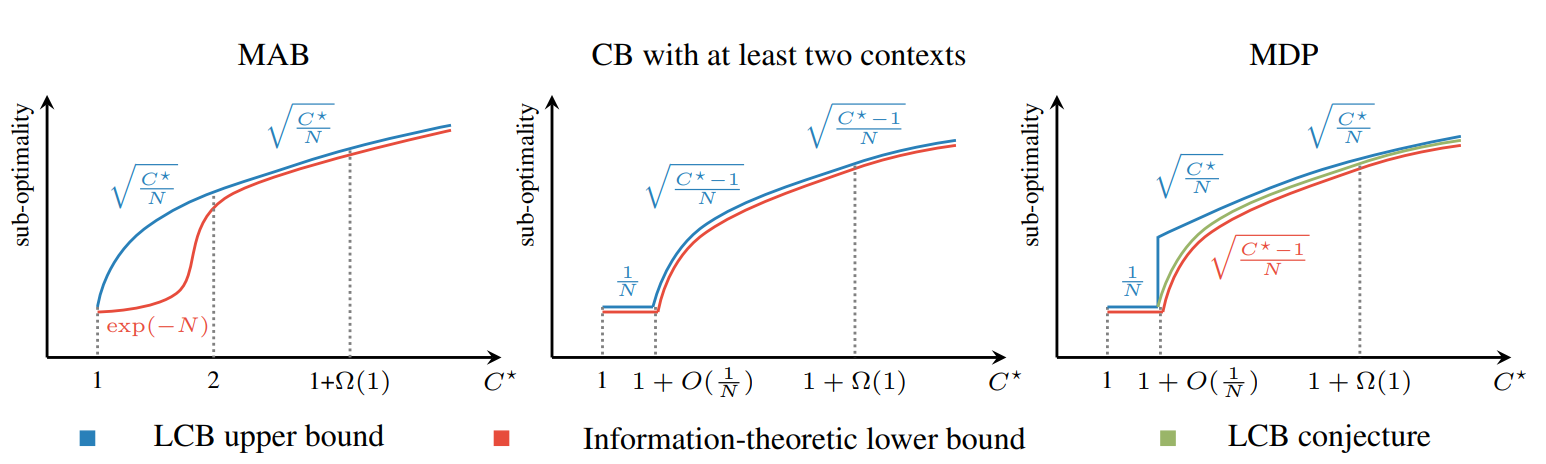
\includegraphics[width=0.8\textwidth]{bridging.png}
  \end{figure}
\end{frame}

\input|"./.venv/bin/python -u scripts/maze_solver_beamer.py"



\end{document}